\subsection{Merge Sort}

\subsubsection{Core concept}
Merge sort uses the powerful strategy of divide and conquer. The array is repeatedly split into smaller subarrays then merging them together. During the merging process, the elements are compared and sorted to create larger sorted subarrays repeat this process until all subarrays are merged back into the original array, resulting in a fully sorted array. By breaking the problem into smaller and then combining the sorted pieces, merge sort efficiently sorts the entire array.

\vspace{3pt}

\subsubsection{Step-by-step Explanations}
\begin{itemize}[label=-]
    \item Step 1: Divide the Array into Subarrays by calling Recursive to split the array into smaller subarrays until each subarray has only 1 or 2 elements. This is achieved by continuously dividing the array into two halves.
    \item Step 2: Start merging the subarrays back together. Create two temporary arrays to hold the elements of the subarrays being merged. Compare the elements from the two temporary arrays and place the smaller element back into the original array. Continue merging and comparing until all elements are sorted and merged back into the original array.
\end{itemize}

\subsubsection{Complexity Analysis}
\textbf{Time complexity analysis: }
\begin{itemize}
    \item Best-case: $O(nlog(n))$
    \item Average-case: $O(nlog(n))$
    \item Worst-case: $O(nlog(n))$
\end{itemize}

\textbf{Space complexity analysis:} $O(n)$ because we have to create the many arrays with sum of these elements is equal to n elements of original array to merge.

\vspace{5pt}

\textbf{An example of merge sort:} ~\cite{ref2}

\begin{figure}[h]
    \centering
    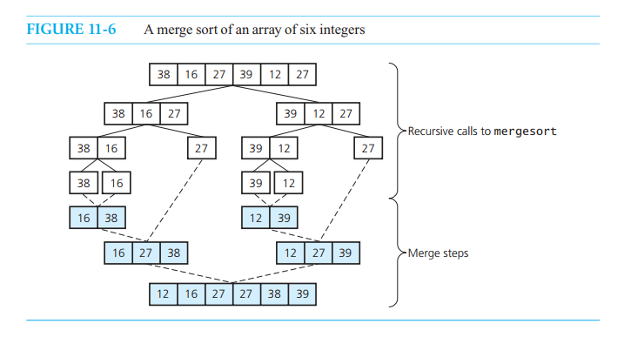
\includegraphics[scale=0.7]{Figures/sort_demo/merge.png}
    \caption{Merge Sort Demo}
    \label{fig:enter-label}
\end{figure}

